%%%
%
% $Autor: Wings $
% $Datum: 2021-05-14 $
% $Pfad: GitLab/MLEdgeComputer/Contents/General/LensCalibrationTool $
% $Dateiname: LensCalibrationTool
% $Version: 4620 $
%
% !TeX spellcheck = de_DE/GB
%
%%%



\chapter{Lens Calibration Tool}


\section{Circle Grid Camera Calibration Patterns}

You can download a PDF version of the circle grid calibration pattern that our SceneScan stereo vision sensor uses for camera calibration. This pattern is compatible to the OpenCV asymmetric circle grid, and can thus also be used for other purposes.
    
When printing the pattern, please ensure that your PDF viewer or printer driver do not scale the document. Otherwise you will not be able to receive accurate metric measurements through stereo vision. You can verify that your printed pattern has the correct scaling, by measuring the reference line at the top of each document.

\begin{figure}
    \begin{center}
        \includegraphics[scale=0.15]{Camera/pattern-a4.pdf}
        
        \caption{Circle Grid Camera Calibration Patterns}
    \end{center}    
\end{figure}

\section{Siemens Star}

The siemens star enables the exact focusing of camera lenses. That is why we print it on the back of our calibration boards. In order to make the camera focusing easier for you as well, you can download our siemens star here.


\begin{figure}
    \begin{center}
        \includegraphics[scale=0.1]{Camera/siemens-star.pdf}
        
        \caption{Siemens Star}
    \end{center}    
\end{figure}

\section{Enjoyyourcamera Testkarte für Kameras und Objektive 30 $\times$ 45 cm}

Testen Sie Ihre Objektive jetzt selbst! Entwickelt vom Tierfotografen Benny Rebel (Bekannt aus Film \& Fernsehen), 400dpi Druck. Testbereiche für Schärfe, Auflösung, Kontrast, Chromatische Abberation, Fokus. Nahtlos erweiterbar für größere Test-Fläche.

Mehrere Testkarten zu einer großen Testkarte zusammenfügbar
Eine Testkarte für Normal- und Teleobjektive, ab 4 Testkarten für Weitwinkelobjektive
Festes Papier, hohe Druckqualität, extrem feine Detailelemente
Einfache Bedienung, Lieferung im stabilen Karton
Sehr viele Testkriterien in einer Karte vereint.


\begin{figure}
    \begin{center}
        \includegraphics[scale=0.1]{Camera/CalibrateCard}
        
        \caption{Siemens Star}
    \end{center}    
\end{figure}

\subsection{Testkarte zum Prüfen von Kameras und Objektiven in Bezug auf ihre Qualität und mögliche Defekte}

Mithilfe dieser von dem Naturfotografen Benny Rebel entwickelten Testkarte lassen sich Kameras und Objektive relativ unkompliziert hinsichtlich ihrer Qualität und möglicher Defekte testen. Damit bietet die Testkarte eine preisgünstige Möglichkeit, die eigene Ausrüstung individuell zu prüfen, und das unabhängig von Testberichten, die wegen einer hohen Serienstreuung bei einigen Objektiv- und Kameramarken oft nicht repräsentativ sind.

\subsection{Zahlreiche Testkriterien: z.B. Schärfe in der Mitte und an den Bildränder, Randabschattungen u.v.m.}

Die Karte deckt zahlreiche Testkriterien ab. Die Kriterien für Kameras sind zum Beispiel die Schärfe in der Bildmitte und an den Rändern, die Auflösung, die Farbwiedergabe, den Kontrastumfang, den Weißabgleich, den Moiré-Effekt, eventuelle Probleme beim automatischen Scharfstellen und das Bildrauschen bei unterschiedlichen ISO-Einstellungen testen. Die Testkriterien für Objektive sind unter anderem Schärfe, Auflösung, Kontrast, Brillanz, Farbwiedergabe, Randabschattungen, chromatische Aberration, Verzeichnung, Vignettierung, eventuelle Probleme beim automatischen Scharfstellen, eine mögliche Dezentrierung der Linsenelemente sowie die Beugung bei unterschiedlichen Blenden.

\subsection{Mehrere Testkarten zu einer großen Testkarte zusammenfügbar - ideal für Weitwinkelobjektive}

Die Testkarte ist so konzipiert, dass man vier oder neun identische Testkarten zu einer großen Testkarte zusammenfügen kann. Für diesen Zweck sind die Testelemente an den Rändern und in den Ecken der Testkarte derart abgeschnitten, dass sie auf einer benachbarten Karte nahtlos weiterverlaufen. Eine große Testfläche, wie sie durch das Zusammenfügen mehrerer Testkarten entsteht, ist wichtig zum Prüfen von weitwinkeligen Objektiven. Solche Objektive besitzen von Natur aus einen weiten Bildwinkel und demzufolge auch einen sehr großen Bildausschnitt. Mit einer großen Testkarte ist sichergestellt, dass die Testfläche den gesamten Bildausschnitt des jeweiligen Objektivs abdeckt, damit man selbst in den Bildecken die Schärfe und andere Kriterien prüfen kann.

\subsection{Eine Testkarte für Normal- und Teleobjektive, vier Testkarten für Weitwinkelobjektive usw.}

Für Normal- und Teleobjektive genügt eine einzelne Testkarte, für Objektive mit einer Brennweite zwischen 50mm und 24mm sollte man vier Testkarten verwenden, und für stark weitwinkelige Objektive mit einer Brennweite von weniger als 24mm empfiehlt sich die Benutzung von 9 Testkarten. Zum Testen von Superweitwinkelobjektiven mit einer Brennweite von weniger als 16mm ergibt es sogar Sinn, die Testkarten nicht direkt aneinanderzufügen. Stattdessen sollte man einen Abstand zwischen den Karten lassen. Wichtig: Die obengenannten Brennweiten beziehen sich auf Objektivtests an Vollformatkameras. Bei Objektivtests an Crop-Kameras verändern sich die Grenzen entsprechend dem Formatfaktor der Kamera. Während man zum Beispiel für ein 35mm-Objektiv an einer Vollformatkamera vier Testkarten benötigt, braucht man für das gleiche 35mm-Objektiv an einer Crop-Kamera mit einem Formatfaktor von 1,5 nur eine Testkarte, denn 35mm x 1,5 ist gleich 52,5mm. Prinzipiell gilt aber: Je größer die Testfläche, desto besser sind die Testergebnisse. Es ergibt also durchaus Sinn, auch zum Testen eines Normalobjektivs vier Testkarten zu verwenden.

\subsection{Festes Papier, hohe Druckqualität, extrem feine Detailelemente für besonders genaues Testen}

Die Testkarte ist auf ein sehr festes, stabiles Papier gedruckt. Außerdem ist die Karte mit einer Druckqualität von 400 dpi extrem detailreich. Die feinsten Detailelemente sind sogar nur einen Punkt breit. Das ermöglicht ein ganz besonders genaues Testen von Objektiv- und Kameraeigenschaften. Außerdem befinden sich die wesentlichen Testflächen sowohl in der Mitte der Karte als auch an den Rändern und in den Ecken. So kann man Eigenschaften wie zum Beispiel die Schärfequalität im gesamten Bildbereich testen. Das hilft dabei, selbst subtile Mängel wie einen Schärfeabfall in den Ecken aufzuspüren.

\subsection{Handhabung}

\begin{enumerate}
  \item Bringen Sie die Testkarte(n) an einer senkrechten, geraden Fläche an. Dafür eignen sich zum Beispiel Holzplatten, gerade Wände oder Glasscheiben. Stellen Sie sicher, dass die Karte gleichmäßig beleuchtet wird, und dass auf der Karte keine Reflexionen zu sehen sind.

  \item Stellen Sie sicher, dass sich die Objektivachse in einem 90 Grad Winkel zur Vorderseite der Testkarte(n) befindet. Richten Sie die Kamera so aus, dass der Bildausschnitt exakt die Testkarte(n) abdeckt. Das Zentrum der Objektivachse sollte genau auf den Mittelpunkt der Testkarte(n) gerichtet sein.

  \item Um ein unverfälschtes Ergebnis zu bekommen, muss die Kamera absolut vibrationsfrei ausgelöst werden. Je nach Brennweite können schon geringe Abweichungen eine Randunschärfe auf dem Foto erzeugen. Benutzen Sie deshalb am besten ein Stativ und einen Fernauslöser. Aktivieren Sie außerdem, sofern vorhanden, die Spiegelvorauslösung. Und deaktieren Sie die Bildstabilisierung.

  \item Für einen Standardtest empfehlen sich folgende Einstellungen:Stellen Sie die Kamera auf Blendenvorwahl (Zeitautomatik) und die Lichtempfindlichkeit auf ISO 200. Wählen Sie idealerweise das Bildformat RAW. Arbeiten Sie außerdem mit dem manuellen Weißabgleich, nach dem Sie diesen auf das Umgebungslicht abgestimmt haben. Für weiterführende Tests, wie zum Beispiel das Bildrauschen bei verschiedenen ISO-Einstellungen, können Sie Einstellungen an der Kamera verändern.

  \item endenreihen: Als erstes Bild bietet sich immer die Offenblende an. Danach kann man der Reihe nach alle Blendenschritte testen (z.B. 1.0 - 1.4 - 2.0 - 2.8 - 4.0 - 5.6, 8.0 - 11 - 16 - 22).

  \item Brennweitenreihen bei Zoom-Objektiven: Auf jeden Fall sollten Sie die Anfangsbrennweite und die Endbrennweite testen. Bei einem 24-70mm Objektiv wären das die Brennweiten 24mm und 70mm. Danach können Sie die Brennweiten in den Schritten testen, wie Sie auch als Festbrennweiten häufig genutzt werden: Das hat den den Vorteil, dass man dann die Abbildungsleistung des jeweiligen Objektivs auch mit der Qualität gängiger Festbrennweiten vergleichen kann.

  \item Und ganz wichtig: Um beim Testen von Wechselobjektiven und Wechselobjektivkameras feststellen zu können, ob ein Defekt vom Objektiv oder von der Kamera ausgeht, sollten Sie Objektive an verschiedenen Kameras testen, und Kameras mit verschiedenen Objektiven. Defekte und Qualitätsmängel müssen nicht zwingend vom Objektiv ausgehen, auch ein schief in der Kamera verbauter Chip kann eine Ursache für eine mangelnde Bildqualität sein.
\end{enumerate}


\bigskip

\section{B.I.G. RES7 Testtafel für Kameras und Objektive}

Die RES7 Testtafel, in der Größe 32x47cm mit matter Oberfläche, wurde für Fotografen entwickelt, um die Bildqualität zu testen und die Grenzen der Auflösung von Kamera und Objektiv beurteilen zu können.

Mit der Tafel kann die Messung der Bildqualität von Digitalkameras, die Messung der Auflösung von optischen Geräten (Vergrößerung 30-50x), die Kontrolle der Belichtung, die grobe Bestimmung gering auflösender Objektive (5-10x) sowie die Kontrolle der Fokussierung und der Schärfentiefe durchgeführt werden.

Die Testtafel eignet sich für Fotokameras bis zu 4000 aktiven Pixeln in der Bildhöhe, d.h. für alle Kompakt-, sowie DSLR- oder DSLM-Kameras mit einer maximalen Auflösung von 24 Megapixeln.

\begin{figure}
    \begin{center}
        \includegraphics[width=0.8\textwidth]{Camera/Testtafel}
        
        \caption{Siemens Star}
    \end{center}    
\end{figure}

\subsection{BIG RES7 Test Board für Kameras und Objektive}
Das BIG RES7 Test Board für Kameras und Objektive in der Größe 32 x 47 cm mit einer matten Oberfläche wurde für Fotografen entwickelt, um die Bildqualität zu testen und die Grenzen der Kamera- und Objektivauflösung abzuschätzen.

Das Board kann zur Messung der Bildqualität von Digitalkameras, zur Messung der Auflösung optischer Geräte (30-50-fache Vergrößerung), zur Kontrolle der Belichtung, zur groben Bestimmung niedrig auflösender Objektive (5-10-fach) und zur Kontrolle von Fokus und Schärfentiefe verwendet werden.

\subsection{Merkmale des BIG RES7 Test Boards für Kameras und Objektive}

\begin{itemize}
  \item Entwickelt für Fotografen zum Testen der Bildqualität
  \item Um die Grenzen der Kamera- und Objektivauflösung abzuschätzen
  \item Um die Bildqualität von Digitalkameras zu messen
  \item Um die Auflösung von optischen Geräten zu messen (Vergrößerung 30-50x)
  \item Matte Oberfläche
  \item Abmessungen: 32 x 47 cm
\end{itemize}


\section{Pattern Generator}

\URL{https://calib.io/pages/camera-calibration-pattern-generator}

\URL{https://markhedleyjones.com/projects/calibration-checkerboard-collection}



Customize a pattern to match your application perfectly and download a printable PDF file. The pattern generator and its outputs can be used for internal development or educational use only. Any commercial purposes or re-sale is strictly prohibited without prior consent. 

NOTE: When printing on a standard inkjet or laser printer, please make sure that your software or printer does not apply any scaling to the pattern. Also make sure that no rasterisation is performed in the printer driver. It is advisable to measure the final pattern after printing.

Once you have settled on a pattern and would like to order a professionally made, highly accurate calibration target, feel free to send us an email at sales@calib.io , and we will happily give you a quote!


\begin{figure}
    \begin{center}
        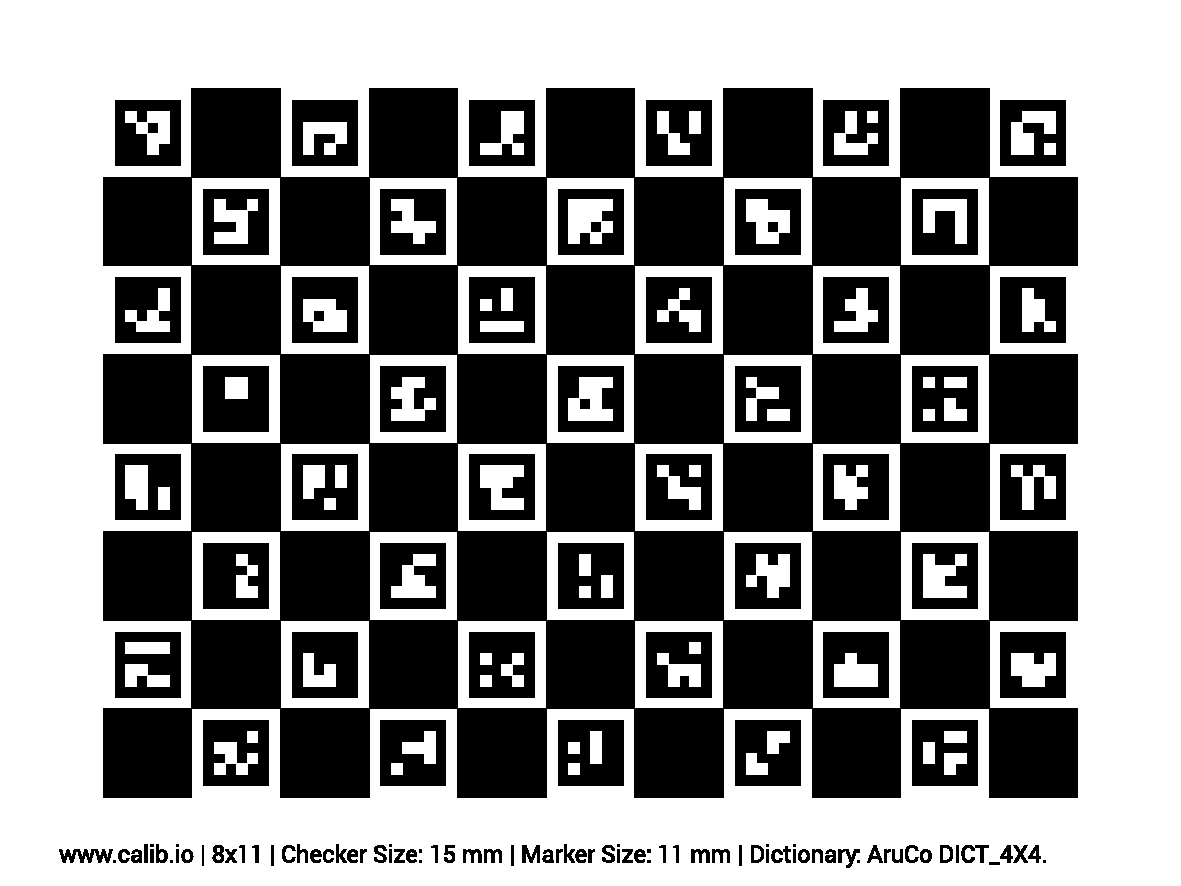
\includegraphics[width=0.8\textwidth]{Camera/calib.io_charuco_200x150_8x11_15_11_DICT_4X4.pdf}
        
        \caption{Siemens Star}
    \end{center}    
\end{figure}


\begin{figure}
    \begin{center}
        \includegraphics[width=0.8\textwidth]{Camera/calib.io_checker_200x150_8x11_15.pdf}
        
        \caption{Siemens Star}
    \end{center}    
\end{figure}


\section{Chess Board}

\cite{Ntouskos:2007}
\cite{Ntouskos:2007a}
\cite{Ntouskos:2009}
\cite{Prokos:2012}

\begin{figure}
    \begin{center}
        \includegraphics[width=0.8\textwidth]{Camera/camera-calibration-checker-board_9x7.pdf}
        
        \caption{Siemens Star}
    \end{center}    
\end{figure}






\section{To Do}

Arducam Lens Calibration Tool, Sichtfeld (Field of View, FoV) Test Chart Folding Card, Pack of 2

\url{https://www.amazon.com/-/de/dp/B0872Q1RLD/ref=sr_1_40?__mk_de_DE=ÅMÅŽÕÑ&dchild=1&keywords=arducam&qid=1622358908&sr=8-40}

\begin{description}
  \item[Multifunktional für Objektiv:] Objektivfokus kalibrieren, FoV messen und Schärfe abschätzen
  \item[Einfach zu bedienen:] Schnelle Einrichtung in Sekunden und Messung in Minuten mit Online-Videotutorial.
  \item[Ein handliches Werkzeug:] Einfaches Ermitteln des Sichtfelds des Objektivs ohne Berechnung
  \item[Sauber und aufgeräumt:] Faltbarer Kartenstil, mehrfach gefaltet und aufgerollt für schnelle Einstellung und bessere Lagerung
  \item[Anwendung:] Fokuskalibrierung, Schärfeschätzung und Bildfeld-Schnellmessung für M12, CS-Mount, C-Mount und DSLR-Objektive.

\end{description}
\url{https://www.arducam.com/product/arducam-lens-calibration-tool-field-of-view-fov-test-chart-folding-card-pack-of-2/}


\begin{figure}
  \begin{center}
    \includegraphics[width=\textwidth]{CAM/LensCalibrationTool/LensCalibrationTool}
    \quad 
    \includegraphics[width=\textwidth]{CAM/LensCalibrationTool/LensCalibrationTool4}
  
    \caption{Kalibrierungswerkzeug der Firma Arducam; \cite{Arducam:2021}}
  \end{center}    
\end{figure}

\section{Übersicht}

Sind Sie immer noch frustriert von der Berechnung des FOV Ihrer Objektive und den unscharfen Bildern? Arducam hat jetzt ein multifunktionales Tool für Objektive veröffentlicht, mit dem Sie das Sichtfeld des Objektivs ohne Berechnung erhalten und den Objektivfokus schnell und einfach kalibrieren können.

\section{Applications}

Focus calibration, sharpness estimation and field of view quick measuring for M12, CS-Mount, C-Mount, and DSLR lenses

\section{Package Contents}

2*Foldable Lens Calibration Card


\subsection{Licht, Farben und Farbmodelle}
{Farbe ist eine Eigenschaft des Lichts, die durch die verschiedenen Wellenlängen des sichtbaren Lichtspektrums entsteht. Farben werden durch das menschliche Auge wahrgenommen, wenn Licht auf Objekte trifft und reflektiert wird. Diese reflektierten Lichtwellen werden von den Photorezeptoren (Zapfen) in der Netzhaut des Auges erfasst und vom Gehirn interpretiert. \cite{Hasche:2016}
    
 Es gibt in der Programmierung verschiedene Farbmodelle, die je nach Anwendungsbereich verwendet werden. Die wichtigsten Farbmodelle sind:}

\subsubsection{Das additive RGB-Farbmodell (Rot, Grün, Blau)}

Die Farben bei dem Farbmodell RGB werden mittels der Farbmischung von Rot, Grün und Blau zusammengesetzt. Mittels dieser drei Grundfarben können verschiedene Kombinationen und damit unterschiedliche Farben erzeugen werden. Mischt man alle Grundfarben, erhält man weiß. Schaltet man alle Grundfarben ab, so erhält man Schwarz.
    Die Grundfarben können Werte zwischen 0 und 255 einnehmen, wodurch die Helligkeit dieser Grundfarbe eingestellt werden kann. \cite{Hasche:2016}

\begin{itemize}
    \item Beispiel: RGB (255, 0, 0) repräsentiert die Farbe Rot.
\end{itemize}



\subsubsection{Das HSV Farbmodel}
{HSV (Hue, Saturation, Value): Ein Farbmodell, das Farben in Bezug auf Farbton, Sättigung und Helligkeit beschreibt. Dieses Modell ist besonders nützlich in der Bildbearbeitung und bei der Farbauswahl, da es eine intuitive Darstellung der Farbkomponenten bietet.
    
    Hue (Farbton): Bestimmt die Grundfarbe und wird in Grad von 0 bis 360 angegeben.\\
    
    Saturation (Sättigung): Bestimmt die Intensität der Farbe und wird als Prozent-\\wert von 0\% (Grau) bis 100\% (voll gesättigte Farbe) dargestellt.\\
    
    Value (Helligkeit): Bestimmt die Helligkeit der Farbe und wird ebenfalls als Prozent-\\wert von 0\% (schwarz) bis 100\% (volle Helligkeit) dargestellt. \cite{Hasche:2016}
    \\
    \textbf{Beispiel:}
}

\begin{itemize}
    \item Hue (Farbton): 0°
    \item Saturation (Sättigung): 50\%
    \item Value (Helligkeit): 100\%  \\
    \\
    Diese Werte beschreiben ein helles Rot im HSV-Farbmodell.
\end{itemize}

\subsubsection{Graustufen}
{Graustufenerkennung bezieht sich auf die Verarbeitung von Bildern, die keine Farbinformationen enthalten, sondern nur Helligkeitswerte. Ein Graustufenbild ist ein Bild, bei dem jeder Pixel einen Helligkeitswert hat, der typischerweise in einem Bereich von 0 (schwarz) bis 255 (weiß) liegt.
    
    Umwandlung von Farbbildern in Graustufenbilder.\\
    
    Farbbilder können in Graustufenbilder umgewandelt werden, indem die Farbkanäle (Rot, Grün und Blau) kombiniert werden, um einen einzelnen Helligkeitswert zu erzeugen. 
    Eine Möglichkeit ist das Umwandeln mit der Durchschnittsmethode, bei dem der  Graustufenwert durch den Durchschnitt der RGB-Werte berechnet wird.
}

\begin{equation}
    Gray = \frac{ R + G + B }{ 3}
\end{equation}

{Um die Wahrnehmungsempfindlichkeit des menschlichen Auges auf Farben zu berücksichtigen, kann folgende Formel verwendet werden:
}

\begin{equation}
    Gray = 0.33 \times R + 0.22\times G+ 0.17\times B
\end{equation}

Dieses Verfahren liefert in der Regel bessere Ergebnisse, da es die menschliche Wahrnehmung besser widerspiegelt. \cite{Hasche:2016}

\newpage
\subsection{Texterkennung}
{Grundsätzlich funktioniert Texterkennung über das sogenannte ``Optical character recognition'' (OCR), hierfür müssen aber erstmal einige Voraussetzungen getroffen werden.}

\subsubsection{Voraussetzungen}
{Das Bild muss begradigt werden, dies kann hier aber vernachlässigt werden, wenn man davon ausgeht, dass die Kamera vorher in der Testumgebung kalibriert wurde.
    \\
    Zudem muss das Bild ggf. in ein binäres schwarz-weiß-Bild umgewandelt werden.
}

\subsubsection{Identifizieren der Buchstabenmatrix}
{Es werden zuerst die einzelnen Zeilen identifiziert, indem nach zwei durchgehenden Reihen weißer Pixel in X-Richtung gesucht wird, zwischen welchen schwarze und weiße Pixel gemischt sind, wie in Abbildung \ref{fig:Zeilenerkennung} zu sehen ist.
}

\begin{figure}
    \centering
    \includegraphics[width=0.5\linewidth]{LensCalibrationTool/LineRecognition.png}
    \caption{Zeilenerkennung}
    \label{fig:Zeilenerkennung}
\end{figure}

{Analog dazu werden auch die einzelnen Buchstaben identifiziert, indem nach zwei, durchgehend weißen Reihen in Y-Richtung gesucht wird, zwischen welchen schwarze und weiße Pixel gemischt sind.
}
\\
{Dann werden die einzelnen Buchstaben in eine binäre Matrix übertragen (siehe Abbildung \ref{fig:Buchstaben in binäre Matrix umwandeln}), um sie im nächsten Schritt analysieren zu können.
}

\begin{figure}
    \centering
    \includegraphics[width=0.5\linewidth]{LensCalibrationTool/LettersInBinaryMatrix.png}
    \caption{Buchstaben in binäre Matrix umwandeln}
    \label{fig:Buchstaben in binäre Matrix umwandeln}
\end{figure}

\subsubsection{Zuordnung der Buchstaben durch Sektionierung}
{Der Mittelpunkt der Buchstabenmatrix wird mithilfe folgender Formel errechnet.}

\begin{equation}
    d\equiv\sqrt{ \left( Y_{2  } -Y_{1}\right)^2+\left(X_{2  } -X_{1}  \right)^2 })     
\end{equation}

Mithilfe des Mittelpunkts wird die Buchstabenmatrix in mehrere kleine Sektionen geteilt, um sie besser analysieren zu können. 


Eine mögliche Unterteilung in Sektionen ist in Abbildung \ref{fig:Sektionierung der Buchstabenmatrix} zu sehen.

\begin{figure}
    \centering
    \includegraphics[width=0.5\linewidth]{LensCalibrationTool/SectioningTheLetterMatrix.png}
    \caption{Sektionierung der Buchstabenmatrix}
    \label{fig:Sektionierung der Buchstabenmatrix}
\end{figure}

{Nun werden die einzelnen Sektionen mit der gleichen Sektion sämtlicher Buchstaben, aus sämtlichen Schriftarten verglichen und dem Buchstaben zugeordnet, der die größte statistische Übereinstimmung hat.
}
\\
\subsubsection{Einfacherer Prozess der Zuordnung}
{Um den Prozess zu vereinfachen, lässt sich die Buchstabenmatrix auch in Quadranten teilen, anstatt der vielen Sektionen, wie in Abbildung \ref{fig:Unterteilung der Buchstabenmatrix in Quadranten} zu sehen.
}

\begin{figure}
    \centering
    \includegraphics[width=0.5\linewidth]{LensCalibrationTool/DivisionOfTheLetterMatrixIntoFourQuadrants.png}
    \caption{Unterteilung der Buchstabenmatrix in Quadranten}
    \label{fig:Unterteilung der Buchstabenmatrix in Quadranten}
\end{figure}
{Um dennoch relativ zuverlässige Ergebnisse zu erhalten, können folgende zwölf Merkmale genutzt werden:\\
    F1 = Summer aller schwarzen Pixel im ersten Quadranten / Summe aller schwarzen Pixel der gesamten Buchstabenmatrix\\
    
    F2 = Summer aller schwarzen Pixel im zweiten Quadranten / Summe aller schwarzen Pixel der gesamten Buchstabenmatrix\\
    F3 = Summer aller schwarzen Pixel im dritten Quadranten / Summe aller schwarzen Pixel der gesamten Buchstabenmatrix\\
    F4 = Summer aller schwarzen Pixel im vierten Quadranten / Summe aller schwarzen Pixel der gesamten Buchstabenmatrix\\
    \\
    F5 = F1 + F2 \\F6 = F2 + F3\\ F7 = F3 + F4\\ F8 = F1 + F4\\ F9 = F2 + F4\\ F10 = F1 + F3\\
    \\
    F11 = Anzahl der Eckpunkte, mithilfe der Harris Corner method\\
    F12 = Anzahl der Pixel, der konvexen Hülle um den Buchstaben / Anzahl der Pixel, der kompletten Buchstabenmatrix. \cite{Jana:2014}
    
    
    
    Dann ist das Verfahren analog zu dem der Sektionierung, es wird nach der höchsten Übereinstimmung aller Merkmale in jedem Quadranten, mit dem gleichen Quadranten sämtlicher Buchstaben, aus sämtlichen Schriftarten, gesucht.
    
    
    \newpage
    \subsection{Kamerakalibrierung mit Schachbrett}
    {Die Kamerakalibrierung ist ein fundamentaler Prozess in der Computer Vision, der darauf abzielt, die Parameter einer Kamera zu bestimmen, um Verzeichnungen zu korrigieren und realitätsgetreue räumliche Informationen aus den aufgenommenen Bildern zu extrahieren. Dies ist essenziell für Anwendungen wie 3D-Rekonstruktion, Robotik, Augmented Reality und maschinelles Sehen.
    }
    
    \subsubsection{Einführung}
    {In der Computer Vision bezeichnet die Kamerakalibrierung den Prozess der Bestimmung der internen und externen Parameter einer Kamera. Die internen Parameter umfassen die Brennweite, den optischen Mittelpunkt und die Verzeichnungskoeffizienten, während die externen Parameter die Position und Orientierung der Kamera im Raum beschreiben. Diese Parameter sind notwendig, um die Geometrie der aufgenommenen Szenen korrekt zu interpretieren. \cite{Ramalingam:2017} Sturm 2017, S. 1311)
    }
    
    \subsubsection{Interne Parameter}
    {Die internen Parameter einer Kamera betreffen die Eigenschaften des Kameraobjektivs und des Bildsensors. Dazu gehören:
        
        Brennweite (f): Bestimmt den Vergrößerungsgrad des Objektivs.
        Optischer Mittelpunkt (cx, cy): Der Punkt auf dem Bildsensor, durch den die optische Achse verläuft.\\
        Verzeichnungskoeffizienten: Korrigieren Verzeichnungen wie die radiale Verzeichnung (siehe Abbildung \ref{fig:Radiale Verzeichnung}) (k1, k2, k3) und tangentiale Verzeichnung (siehe Abbildung \ref{fig:Tangentiale Verzeichnung}) (p1, p2).\\
        Die Kalibrierung dieser Parameter erfolgt typischerweise durch die Aufnahme mehrerer Bilder eines bekannten Kalibrierungsmusters, wie z. B. eines Schachbrettmusters, aus verschiedenen Blickwinkeln. Die Beziehung zwischen den erkannten Punkten im Bild und den bekannten 3D-Koordinaten des Musters ermöglicht die Schätzung der internen Parameter. \cite{Grossberg:2001}
    }
    
    \begin{figure}
        \centering
        \includegraphics[width=0.5\linewidth]{LensCalibrationTool/RadialDistortion.png}
        \caption{Radiale Verzeichnung} %(J. Zhang)}
        \label{fig:Radiale Verzeichnung}
    \end{figure}
    
    \begin{figure}
        \centering
        \includegraphics[width=0.5\linewidth]{LensCalibrationTool/TangentialDistortion.png}
        \caption{Tangentiale Verzeichnung} % (J. Zhang)}
        \label{fig:Tangentiale Verzeichnung}
    \end{figure}
    
    \subsubsection{Externe Parameter}

Die externen Parameter beschreiben die Transformation von dem Weltkoordinatensystem zum Kamerakoordinatensystem, bestehend aus:
        
  \begin{itemize}
    \item Rotation (R): Beschreibt die Orientierung der Kamera.
    \item Translation (t): Beschreibt die Position der Kamera im Raum.
    \item Diese Parameter werden ebenfalls durch die Aufnahme mehrerer Bilder eines Kalibrierungsmusters bestimmt, wobei die Positionen des Musters relativ zur Kamera variiert werden.
  \end{itemize}        

    
    \subsubsection{Zhang-Kalibrierungsmethode}
    
    {Ein gängiges Verfahren zur Kamerakalibrierung ist die Verwendung der Zhang-Kalibrierungsmethode, die eine lineare und nicht lineare Optimierung kombiniert, um die Kalibrierungsparameter präzise zu bestimmen. Diese Methode besteht aus folgenden Schritten:\Mynote{citations}
    }
    
    \begin{enumerate}
        \item Bildaufnahme: Mehrere Bilder des Kalibrierungsmusters aus unterschiedlichen Perspektiven
        \item Merkmalserkennung: Identifikation und Zuordnung der Merkmale (Eckpunkte des Schachbrettmusters).
        \item Berechnung der Homografie: Bestimmung der Projektionsmatrix, die die Beziehung zwischen 2D-Bildpunkten und 3D-Weltpunkten beschreibt.
        \item Schätzung der initialen Parameter: Lineare Schätzung der internen und externen Parameter basierend auf den Homografien.
        \item Nicht lineare Optimierung: Feinabstimmung der Parameter durch Minimierung der Reprojektionsfehler.
    \end{enumerate}
    
    
    \subsubsection{Anwendung in der Praxis}
    Eine genaue Kamerakalibrierung ist entscheidend für die Präzision in vielen Anwendungen der Computer Vision:
    
    \begin{itemize}
        \item 3D-Rekonstruktion: Erzeugung akkurater 3D-Modelle aus 2D-Bildern.
        \item Robotik: Präzise Navigation von Robotern.
        \item Augmented Reality: Überlagerung digitaler Inhalte auf reale Szenen in korrekter Perspektive.
        \item Maschinelles Sehen: Erkennung und Verfolgung von Objekten in Bildern und Videos.
    \end{itemize}
    

    \subsection{Kamerakalibrierung mit Farbpaletten}
    Die Farbkamerakalibrierung mit Farbpaletten, siehe Abbildung \ref{fig:Farbpalette}, ist eine zentrale Technik in der Bildverarbeitung, welche darauf abzielt, die Farbwiedergabe von Kameras zu standardisieren und zu verbessern. Diese Methode nutzt standardisierte Farbpaletten, um die Kameras so einzustellen, dass sie Farben präzise und realitätsgetreu wiedergeben. Diese Technik ist besonders in Bereichen wichtig, in denen Farbtreue entscheidend ist, wie in der medizinischen Bildgebung, Qualitätskontrolle und Farbmessung.
    
    \begin{figure}
        \centering
        \includegraphics[width=0.5\linewidth]{LensCalibrationTool/ColorPlates.png}
        \caption{Farbpalette}
        \label{fig:Farbpalette}
    \end{figure}
    
    \subsubsection{Methodik}
    \begin{enumerate}
        \item \textbf{Aufnahme der Farbpalette}
        
        Der erste Schritt in der Kalibrierung besteht darin, Bilder der Farbpalette unter verschiedenen Beleuchtungsbedingungen aufzunehmen. Dies kann sowohl unter natürlichen als auch unter künstlichen Lichtquellen erfolgen. Wichtig ist, dass die Palette flach und gleichmäßig beleuchtet ist, um Verzeichnungen zu vermeiden.
        \item \textbf{Identifikation der Farbfelder}
        
        Nach der Aufnahme werden die einzelnen Farbfelder in den Bildern identifiziert. Dies kann manuell oder automatisch erfolgen, wobei Algorithmen zur Mustererkennung verwendet werden, um die Positionen der Farbfelder zu bestimmen.
        \item \textbf{Vergleich mit Referenzwerten}
        
        Die im Bild gemessenen Farbwerte der einzelnen Felder werden mit den bekannten Referenzwerten der Farbpalette verglichen. Dies geschieht häufig im CIE-Lab-Farbraum, der eine perpetuell Farbskala mit gleichem Abstand bietet.
        \item \textbf{Berechnung der Transformationsmatrix}
        
        Basierend auf den Differenzen zwischen den gemessenen und den \\Referenzfarbwerten wird eine Farbtransformationsmatrix berechnet. Diese Matrix dient dazu, die Farbabweichungen zu korrigieren und die Kamera so zu kalibrieren, dass sie die Farben korrekt wiedergibt.
        \item \textbf{Anwendung der Farbkorrektur}
        
        Die berechnete Transformationsmatrix wird dann auf alle zukünftigen Bilder angewendet, die mit der kalibrierten Kamera aufgenommen werden. Dies stellt sicher, dass die Farben in diesen Bildern den Referenzfarben entsprechen.
        
    \end{enumerate}
    
    \subsubsection{Herausforderungen}
    \begin{itemize}
        \item \textbf{Beleuchtungseinflüsse}
        
        Eine der größten Herausforderungen bei der Farbkamerakalibrierung ist die Variabilität der Beleuchtung. Unterschiedliche Lichtquellen können die Farbwahrnehmung erheblich beeinflussen. Eine Lösung besteht darin, die Kalibrierung unter verschiedenen Beleuchtungsbedingungen durchzuführen und Beleuchtungskorrekturfaktoren zu entwickeln.
        \item \textbf{ Alterung der Farbpaletten}
        
        Farbpaletten können mit der Zeit verblassen oder sich verändern, was die Genauigkeit der Kalibrierung beeinträchtigen kann. Regelmäßige Überprüfungen und der Austausch der Farbpaletten sind notwendig, um eine konstante Kalibrierung zu gewährleisten.
        \item \textbf{Kamera interne Verarbeitung}
        
        Moderne Kameras führen oft interne Bildverarbeitungen durch, die die \\Rohdaten verändern. Um dies zu umgehen, sollte die Kalibrierung möglichst auf den Rohdaten (RAW) der Kamera basieren und die Kamera interne \\Farbkorrekturen deaktiviert werden.
    \end{itemize}
    

    \subsection{Bibliotheken in der Programmierung}
    
In der Programmierung bezeichnet man Bibliotheken, eine Sammlung  von Unterprogrammen, die Lösungswege für thematisch zusammengehörende Problemstellungen anbieten. Im Gegensatz zu eigenständig lauffähigen Programmen sind Bibliotheken keine eigenständigen Einheiten. Stattdessen enthalten sie Hilfsmodule, die von anderen Programmen angefordert werden. 
    
    Es ist sinnvoll Bibliotheken zu nutzen, da man thematisch ähnliche Programme nutzen kann und auf seine eigenen Programme anwenden kann. Durch die Nutzung von bereits bestehenden Programmen kann zeitsparend gearbeitet werden.
    
    
\bigskip
    
    
    Verwendete Bibliotheken sind:


\subsubsection{Tkinter}
\PYTHON{Tkinter} ist eine Bibliothek, die es ermöglicht, grafische Benutzeroberflächen (GUIs) zu erstellen. Mithilfe von \PYTHON{Tkinter} lassen sich leicht Fenster, Schaltflächen, Textfelder und viele andere GUI-Elemente erstellen. Mit der Funktion Fenster lassen sich Hauptfenster und Dialogfenster erstellen. Widgets wie Schaltflächen, Textfelder, Listenfelder und Radiobuttons können mit \PYTHON{Tkinter} erstellt werden. Außerdem kann man mit \PYTHON{Tkinter} das Layout der verwendeten Widgets wie die Positionen und das Aussehen individuell einstellen. Es können Befehle und Ereignisse wie Mausklicks und Tastatureingaben eingebaut werden, die das Steuern von gewissen Befehlen ermöglichen. 

\bigskip

\textbf{Benutzeroberfläche}

Mit der Bibliothek Tkinter können Benutzeroberflächen erstellt werden. In diesem Fenster können unterschiedliche Widgets eingebaut werden. Der folgende Code zeigt einen grundlegenden Aufbau einer Benutzeroberfläche.

\bigskip

\PYTHON{app = tk.Tk()}

\PYTHON{app.title("Fenstername")}

\PYTHON{app.geometry("400x300")}

\PYTHON{app.mainloop()}

\bigskip


In dem Code ist \PYTHON{app} die Variable, die auf das Hauptfensterobjekt verweist. In der ersten Zeile wird ein neues Hauptfenster erstellt. Mithilfe von \PYTHON{app.title} kann der Name des Fensters geändert werden.
    
In der dritten Zeile kann die Größe (x-Richtung, y-Richtung) des Fensters verändert werden. In der vierten Zeile wird \PYTHON{app.mainloop()} eingebaut, wodurch das Fenster dauerhaft geöffnet bleibt, bis es geschlossen wird. Ohne diese Eingabe würde sich das Hauptfenster nach kurzer Zeit schließen. Es gibt noch weitere Einstellungen, womit das Hauptfenster bearbeiten werden kann.

\bigskip

\textbf{Bedienung des Benutzers}

Mit der Bibliothek Tkinter können Buttons erstellt werden, wodurch die Bedienung durch den Benutzers ermöglicht wird. Der folgende Code zeigt den grundlegenden Aufbau eines Buttons:

\bigskip


\PYTHON{def button1():}
\PYTHON{\qquad print("Button clicked!")}

\PYTHON{\qquad button = tk.Button(root, text="Click Me", command=button1)}

\PYTHON{\qquad button.pack()}

\bigskip

Zunächst wird eine Funktion mit dem Schlüsselwort \PYTHON{def}, gefolgt vom Namen der Funktion und runden Klammern, erstellt. Innerhalb der Funktion können Befehle definiert werden, die jederzeit ausgeführt werden können. Im Sample wird der Text \PYTHON{Button Clicked!} in der Konsole ausgegeben. Innerhalb der runden Klammern können zudem noch Parameter eingeführt werden, die als Variablen innerhalb der Funktion dienen.  

Nachdem definiert ist, was passiert, wenn die Funktion ausgeführt wird, muss ebenfalls definiert werden, wann die Funktion aktiviert wird.
Dazu wird, mithilfe von \PYTHON{Tkinter}, ein Button erstellt. Die Position, das Aussehen und der ausgeführte Command muss hierfür definiert werden. Im Sample bezieht sich \PYTHON{root} auf das Hauptfenster, in dem alle Widgets (auch Buttons) platziert werden. Als Nächstes wird der Name, der auf dem Button steht, mit \PYTHON{text=} benannt. Am Ende wird der Befehl mit \PYTHON{command=} definiert, welcher bei der Aktivierung des Buttons ausgeführt wird. Im Sample wird die Funktion \PYTHON{button1} ausgeführt.




\subsubsection{OpenCV}

\textbf{OpenCV} ist eine Bibliothek für die Bildverarbeitung und Computer Vision. Funktionen für die Bildverarbeitung sind zum Beispiel die Analyse von Bildern, sowie die Veränderung und Verbesserung dieser.

Mithilfe von Computer Vision-Aufgaben lässt sich Visualisierung der Umgebung erlernen. Es hilft dabei, Bilder zu verarbeiten, Objekte zu erkennen, Gesichter zu identifizieren und Bewegung zu verfolgen.\\
Da das Erstellen von Programmen mit Bildverarbeitung zeitlich aufwendig werden kann, ist es sinnvoll bereits bestehende Unterprogramme für die eigene Nutzung zu verwenden.\\

\newpage

\textbf{Kameraübertragung}\\

cap = cv2.VideoCapture(0)\\
\\
if not cap.isOpened():\\
print("Fehler: Kamera konnte nicht geöffnet\\ werden.")\\
exit()\\
\\
while True:\\
ret, frame = cap.read()\\
\\
if not ret:\\
print("Fehler: Frame konnte nicht gelesen\\ werden.")\\
break\\
\\
cv2.imshow('Kamera', frame)\\
\\
if cv2.waitKey(1) \\
if key == 27:\\
break\\
\\
cap.release()\\
cv2.destroyAllWindows()\\


Die erste Zeile öffnet die Kamera. Die Auswahl der Kamera kann mit der runden Klammer gesteuert werden. Die Zahl Null in den runden Klammern steht für die erste angeschlossene Kamera. Die dritte Zeile überprüft, ob die Kamera geöffnet werden kann. Wenn sie nicht geöffnet werden, wird eine Fehlermeldung ausgegeben und das Programm wird mit "exit()" beendet. Als Nächstes wird eine Schleife verwendet, um fortlaufende Frames zu lesen. Der Wert "ret" gibt an, ob das Lesen funktioniert hat und "frame" enthält das aktuelle Bild. Zeile zehn überprüft, ob der aktuelle Frame erfolgreich gelesen werden konnte. War die Überprüfung nicht erfolgreich, wird eine Fehlermeldung ausgegeben und die Schleife wird beendet. Die Zeile 14 zeigt den aktuellen Frame in einem Fenster an. Im Sample wird das Bild in dem Fenster "Kamera" wiedergegeben. Als Nächstes erfolgt eine Überprüfung der Tasteneingabe, wodurch die Schleife und damit auch die Bildanzeige geschlossen werden kann. Im Sample wird überprüft, ob die Taste "Esc" gedrückt wurde, wodurch die Schleife beendet werden würde. Die letzten beiden Zeilen des Codes geben die Kamera frei und schließen alle geöffneten Fenster, sobald das Programm abgebrochen wird.\\
\newpage

\textbf{Bilderfassung}\\

if key == ord('c'):  \\
filename = "captured\_image.png" \\
cv2.imwrite(filename, frame) \\
print(f"Bild wurde als {filename} \\ gespeichert.")            \\
break\\


Der Code startet mit einer Bedingung, bei der überprüft wird, ob die Taste "c" gedrückt wurde.
Wird die Taste "C" gedrückt, wird der folgende Code ausgeführt. Zuerst wird der Dateiname des Bildes festgelegt, um das aufgenommene Bild zu speichern. Der Frame, welcher bei der Eingabe zu sehen war, wird als Bild mit dem Dateinamen "filename" gespeichert. Daraufhin erfolgt eine Bestätigung in der Konsole und die aktuelle Schleife wird mit "break" beendet.\\

\textbf{Bildspeicherung}\\

filename =\\ f"captured\_image\_{datetime.now().strftime("")}\\.png" 
cv2.imwrite(filename, frame)\\
print(f"Bild gespeichert als {filename}")\\


In der ersten Zeile wird der Dateiname erstellt, der das Datum und die Uhrzeit der Bildaufnahme enthält. In der zweiten Zeile wird das aufgenommene Bild ge-\\speichert. Der Name der Datei ist \glqq filename\grqq{}, in die das Bild gespeichert werden soll. Der Name \glqq frame\grqq{} bezeichnet das Bild, das gespeichert werden soll. Das Bild wurde vorher mit \glqq ret, frame = cap.read()\grqq{} aufgenommen und in der Variable \glqq frame\grqq{} gespeichert.\\

\newpage

\textbf{Farberkennung}\\

hsv\_frame = cv2.cvtColor(frame,\\ cv2.COLOR\_BGR2HSV)\\
\\
height, width, \_ = frame.shape\\
\\
cx = int(width / 2)\\
cy = int(height / 2)\\
\\
pixel\_center = hsv\_frame[cy, cx]\\
hue\_value = pixel\_center[0]\\
\\
color = "Undefined"\\
if hue\_value < 5:\\
color = "RED"\\
elif hue\_value < 78:\\
color = "GREEN"\\
elif hue\_value < 131:\\
color = "BLUE"\\
\\
else:\\
color = "RED"\\

pixel\_center\_bgr = frame[cy, cx]\\
b, g, r = int(pixel\_center\_bgr[0]),\\ int(pixel\_center\_bgr[1]),\\
int(pixel\_center\_bgr[2])\\
\\
cv2.rectangle(frame, (cx - 220, 10), (cx + 200, 120),
(255, 255, 255), -1)\\
cv2.putText(frame, color, (cx - 200, 100), 0,\\ 3, (b, g, r), 5)\\
cv2.circle(frame, (cx, cy), 5, (25, 25, 25), 3)\\
\\
cv2.imshow("Frame", frame)\\
key = cv2.waitKey(1)\\
if key == 27:\\
break\\


In dem Code wird die Farbe eines Pixels im Zentrum der Kamera analysiert und die erkannte Farbe angezeigt.
Der Code beginnt mit der Konvertierung des Bildes von BGR (Blue, Green, Red) zu HSV (Hue, Saturation, Value) Farbschema. Durch die Konvertierung wird die Analyse der Farbe erleichtert, da im HSV-Farbmodell der Farbton getrennt von der Helligkeit betrachtet wird. Als Nächstes wird die Höhe, Breite und die Anzahl der Farbkanäle des Bildes bestimmt. Daraufhin werden die X- und Y-Koordinaten des Bildzentrums berechnet, damit im folgenden Schritt der HSV-Wert des zentralen Pixels extrahiert werden kann. Aus dem HSV-Wert wird der Farbton (Hue) des zentralen Pixels extrahiert. Als Nächstes folgt eine Überprüfung unterschiedlicher Bedingungen, um den Farbtonwert "hue\_value" zu analysieren und die Farbe entsprechend einzuteilen. Die Einteilung der Farben entspricht den Farbtönen im HSV-Farbmodell.\\
Außerdem wird der BGR Wert des zentralen Pixels des Bildes bestimmt, um die Textausgabe auf die entsprechende Farbe abzugleichen. 
Die nächsten Zeilen im Code dienen dazu, ein Kreis in der Mitte des Bildes einzufügen, welcher für die Bestimmung der Farbe ausgewählt wurde. Außerdem wird in der oberen linken Ecke ein Text mit dem erkannten Farbnamen eingefügt. Am Ende kann das Programm wieder mit der Tasteneingabe "Esc" beendet werden.\\


\textbf{Graustufenerkennung}\\

def graustufe\_prozent(image, x, y):\\
gray\_image = cv2.cvtColor(image,\\ cv2.COLOR\_BGR2GRAY)\\
grayscale\_value = gray\_image[y, x]\\
grayscale\_percentage = (255 -\\ grayscale\_value) / 255 * 100\\
return grayscale\_percentage\\
\\
def graustufenerkennung(kamera\_nummer=1):\\
cap = cv2.VideoCapture(kamera\_nummer)\\
\\
while True:\\
ret, frame = cap.read()\\
if not ret:\\
break\\
\\
height, width, \_ = frame.shape\\
center\_x, center\_y = width // 2, height // 2\\
\\
grayscale\_percentage =\\ get\_grayscale\_percentage\\
(frame, center\_x, center\_y)\\
\\
grayscale\_text = f"Graustufenwert:\\ {grayscale\_percentage:.2f}\%"\\
\\
cv2.circle(frame, (center\_x, center\_y), 5,\\ (0, 255, 0), 2)\\
text\_color = (200, 100, 0)  \\
\\
cv2.putText(frame, grayscale\_text, (10, 30),\\ 
cv2.FONT\_HERSHEY\_SIMPLEX, 0.7, text\_color, 2, cv2.LINE\_AA)\\
\\
cv2.imshow('Grayscale Detection', frame)\\
\\
if cv2.waitKey(1) \& 0xFF == ord('27'):\\
break\\
\\
cap.release()\\
cv2.destroyAllWindows()\\


Die Funktion "graustufe\_prozent" konvertiert das aktuelle Bild in Graustufen um. Der Graustufenwert der Pixel an den voreingestellten Koordinaten (x,y) wird bestimmt und dann der Graustufen-Prozentsatz (0\% für Weiß und 100\% für Schwarz) berechnet. Die Hauptfunktion "graustufenerkennung" öffnet die Kamera und erfasst, während die Schleife läuft, dauerhaft Frames aus dieser Quelle. Für jedes erfasste Frame wird im folgenden Schritt der Graustufen-Prozentsatz in der Mitte des Bildes, mithilfe der ersten Funktion, berechnet und angezeigt. Die Schleife, und damit das Programm, können mittels der Tasteneingabe "Esc" geschlossen werden.\\


\subsubsection{Easyocr}
\textbf{Easyocr} ist eine Python-Bibliothek, die OCR (Optical Character Recognition) Funktionalität bietet. Der Import von Easyocr ermöglicht es, OCR im Python-Code zu verwenden, um Text aus Bildern zu extrahieren.\\


\textbf{Texterkennung}\\


reader = easyocr.Reader(['de'])\\
\\
result = reader.readtext(image)\\
\\
print("Erkannter Text im Bild:")\\
for (bbox, text, prob) in result:\\
print(f"{text} (Wahrscheinlichkeit:\\ {prob:.2f})")\\
\\
img\_with\_text = np.copy(image)\\
for (bbox, text, prob) in result:\\
\\
cv2.putText(img\_with\_text, text,\\ (int(bbox[0][0]), \\
int(bbox[0][1]) - 10),\\
cv2.FONT\_HERSHEY\_SIMPLEX, 1, (0, 255, 0), 2)\\



In der ersten Zeile wird ein Easyocr-Objekt initialisiert, das darauf trainiert ist, Text in Bildern zu erkennen. In den eckigen Klammern kann die Sprache, des zu erkennenden Textes, eingestellt werden. Das "de" wird benötigt, damit deutschsprachige Texte erkannt werden. Im nächsten Schritt wird das übertragene Bild \\"image" auf Text analysiert, welches in der Variable "result" gespeichert wird. Dabei handelt es sich um eine Liste von Tuplen, wobei jede Tuple, den Begrenzungsrahmen, den erkannten Text und die entsprechende Wahrscheinlichkeit enthält. Die Informationen aus jeder Tuple werden mithilfe einer Schleife durchlaufen und ausgegeben. Als Nächstes wird eine Kopie des Originalbildes erstellt, um den erkannten Text darauf abzubilden. Mithilfe einer weiteren Schleife wird jedes Tuple durchgegangen und Informationen auf das Bild übertragen.


\subsubsection{Datetime}
Die Bibliothek Datetime in Python bietet eine Reihe von Funktionen, die es ermöglichen, mit Datums- und Zeitangaben zu arbeiten.\\


f"captured\_image\_{datetime.now().strftime('\% Y\%m\%d\%H\%M\%S')}.png"\\


Die gegebene Zeile erzeugt einen Dateinamen für ein Bild, welches das aktuelle Datum und die aktuelle Uhrzeit enthält.

\subsubsection{Numpy}
Die Bibliothek Numpy ist eine leistungsstarke Bibliothek für numerische Berechnungen. Sie bietet Unterstützung für große, mehrdimensionale Arrays und Matrizen, zusammen mit einer Vielzahl von mathematischen Funktionen, um effizient über diese Arrays zu arbeiten.\\

\textbf{Texterkennung}\\

img\_with\_text = np.copy(image)\\


Im Abschnitt der Texterkennung wird die Bibliothek Numpy verwendet, um eine Kopie des Bildes zu erstellen, damit das Originalbild unverändert bleibt, während der erkannte Text in die Kopie übermittelt wird.\\


\textbf{Kalibrierung}\\


objp = np.zeros((chessboard\_size[0] *\\ chessboard\_size[1], 3), \\
np.float32)\\
objp[:, :2] = np.mgrid[0:chessboard\_size[0], \\
0:chessboard\_size[1]].T.reshape(-1, 2)\\
\\
np.savez('calibration\_data.npz',\\ **calibration\_data)\\
\\
data = np.load('calibration\_data.npz')\\
\\
known\_colors = np.array([
[115, 82, 68], [194, 150, 130], [98, 122,\\ 157], [87, 108, 67], ...],  dtype=np.float32)\\


Im Abschnitt der Kalibrierung wird die Bibliothek Numpy verwendet, um zuerst die bekannten 3D-Koordinaten, der Schachbrett-Eckpunkte, im Raum darzustellen. Dabei wird Numpy verwendet, da die Arbeit mit vielen Datenpunkten effektiver durchgeführt werden kann.\\ Als Nächstes wird Numpy verwendet, um die Kalibrierungsdaten zu speichern und zu laden. Die Kalibrierungsdaten (Kameramatrix und Verzeichnungskoeffizienten) werden in einer komprimierten ".npz"-   
Datei gespeichert. Außerdem wird die Bibliothek verwendet, damit die bekannten Farben der Colorcards in einem mehrdimensionalen Array gespeichert werden können.  

\newpage

\subsubsection{Os}
Die Bibliothek Os bietet eine Vielzahl von Funktionen zum Interagieren mit dem Betriebssystem. Diese Funktionen ermöglichen es, Dateisystemoperationen, Umgebungsvariablen und Prozesse zu verwalten.\\


directory = "dateipfad"\\
if not os.path.exists(directory):\\
os.makedirs(directory)\\
\\
filename = os.path.join(directory, \\
f"captured\_image\_{datetime.now().strftime('\%Y\%m\%d\%H\%M\%S')}.png")\\
cv2.imwrite(filename, img\_with\_text)\\
print(f"Bild mit erkanntem Text wurde\\ gespeichert als {filename}.")\\


Der Code beginnt mit der Überprüfung, ob das Verzeichnis "directory" existiert. Falls es nicht existiert, wird es von "os.makedirs(directory) erstellt. Als Nächstes wird das Verzeichnis mit dem Dateinamen zu einem vollständigen Pfad verbunden. Dann wird das Bild, mithilfe der OpenCV Bibliothek, gespeichert. Am Ende wird eine Bestätigungsnachricht ausgegeben.  